

\section{Introduction}

Generative models have made significant progress in creating images and videos from text~\citep{song2020denoising,dhariwal2021diffusion,peebles2023scalable,ho2022video,esser2023structure}. A key technique they use is classifier-free guidance (CFG)~\citep{ho2022classifier}, which adjusts the model's output to better match the text prompt. However, using strong guidance can sometimes reduce stability, potentially leading to issues like oversaturated colors or unnatural structures~\citep{karczewski2024diffusion,sadat2024eliminating}. These problems are often more noticeable in modern, high-dimensional models, where using guidance scale without careful adjustment may strongly affect visual quality.

Recent studies have analyzed the stability and mechanisms of guidance strategies~\cite{lin2024common, wang2025foresight}. As models scale to latent spaces with millions of dimensions, they encounter challenges associated with high-dimensional spaces. In such environments, the initial noise magnitude naturally scales with dimensionality~\cite{debortoli2022riemannian}. Our analysis indicates that specifically at the initial timestep of generation, guidance update (difference between the conditional and unconditional model outputs) shares a similar direction across samples. In high-dimensional settings, forcing such a generic direction with a large guidance scale across diverse initial noises can destabilize the early generation trajectory, leading to severe overshooting and deviation from the realistic data distribution.

To address this, we propose \mtd. This method automatically adjusts the guidance scale by comparing it to the model's inherent denoising activity. When guidance is very strong relative to the denoising process, \mtdbk temporarily reduces the guidance scale, which helps keep the generation process stable in the early stages, while allowing a larger guidance scale later when the tones and structures of the image are clearer. The method is designed to be simple with almost no additional computational overhead, and to be compatible with various existing models and other CFG optimization strategies.

Our adaptive guidance schedule aims to accelerate conditional generation while maintaining sample quality, as suggested by metrics like ImageReward, CLIPScore, and vBench. Experiments indicate that \mtdbk can achieve faster inference on models such as SD3.5~\citep{esser2024scalingrectifiedflowtransformers}, Lumina~\citep{gao2024lumina}, and Wan2.1-14B~\citep{wan2.1} compared to baselines. Specifically, results show up to \textbf{3$\times$} acceleration on SD3.5, \textbf{4$\times$} on Lumina, and \textbf{2$\times$} on Wan2.1-14B, while achieving comparable or better performance than their slower baselines. The method also appears robust to hyperparameter settings and applicable across different model scales and domains. Moreover, \mtdbk is orthogonal to other guidance optimization methods, such as Guidance Rescale~\cite{lin2024common} and Adaptive Projection Guidance~\cite{sadat2024eliminating}, enabling seamless integration for cumulative benefits.

In summary, our main contributions are as follows:
\begin{itemize}
   \item We analyze the impact of early-step guidance in flow-based models, supported by theoretical motivation and empirical observations.
   \item We introduce a practical, magnitude-aware adaptive guidance schedule that aims to balance guidance scale across sampling steps.
   \item Through experiments on image and video generation, we demonstrate that our approach can facilitate speedups while maintaining the quality compared to standard CFG, with broad compatibility.
\end{itemize}

\label{sec:exp_video}
\begin{figure*}[t]
    \centering
    % Column Headers
    \begin{minipage}{\linewidth}
        \centering
        \begin{minipage}{0.24\linewidth} \centering \small Resolution: 256 \end{minipage}%
        \hfill
        \begin{minipage}{0.24\linewidth} \centering \small Resolution: 512 \end{minipage}%
        \hfill
        \begin{minipage}{0.24\linewidth} \centering \small Resolution: 768 \end{minipage}%
        \hfill
        \begin{minipage}{0.24\linewidth} \centering \small Resolution: 1024 \end{minipage}
    \end{minipage}
    \vspace{2pt}

    % % Row 1: Sample 1 (Pirate) Original
    % \begin{subfigure}{\linewidth}
    %     \centering
    %     
\includegraphics[width=0.24\linewidth]{fig_tab/007109-0002_org_step10_res256.pdf}
    %     \hfill
    %     
\includegraphics[width=0.24\linewidth]{fig_tab/007109-0002_org_step10_res512.pdf}
    %     \hfill
    %     
\includegraphics[width=0.24\linewidth]{fig_tab/007109-0002_org_step10_res768.pdf}
    %     \hfill
    %     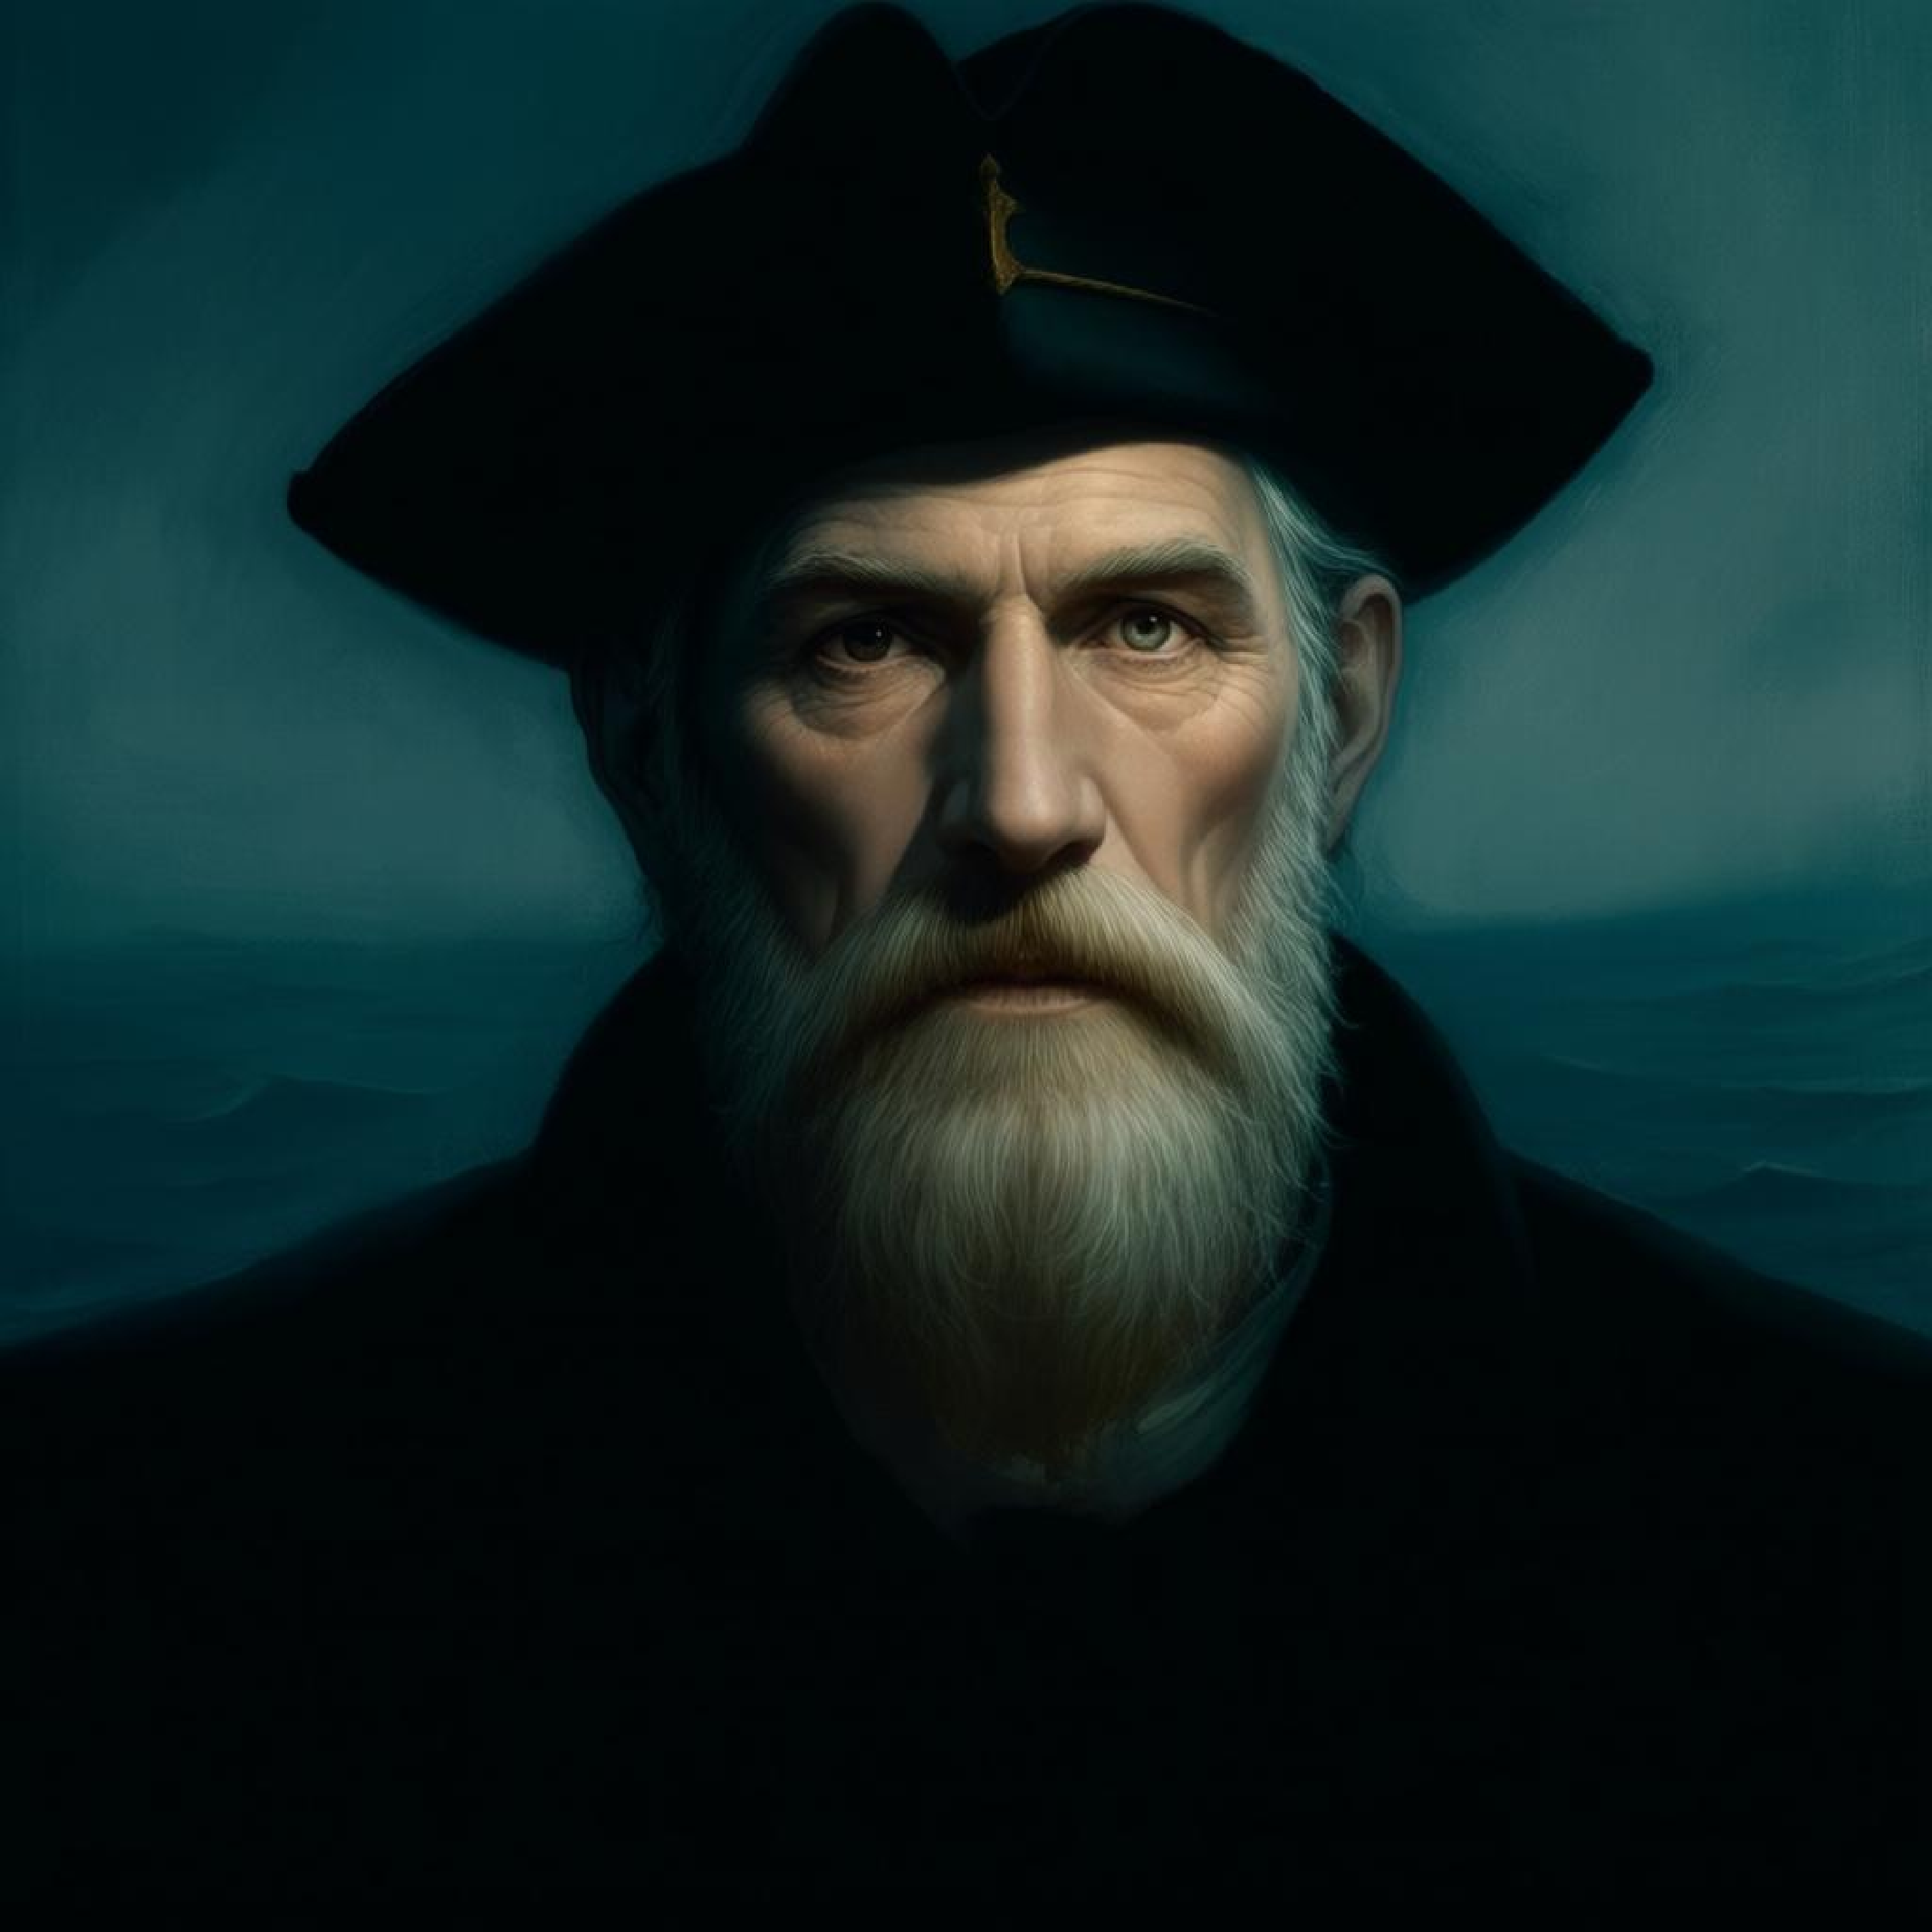
\includegraphics[width=0.24\linewidth]{fig_tab/007109-0002_org_step10_res1024.pdf}
    %     \caption{Pirate: Original}
    % \end{subfigure}
    % \vspace{2pt}

    % % Row 2: Sample 1 (Pirate) MAMBO-G
    % \begin{subfigure}{\linewidth}
    %     \centering
    %     
\includegraphics[width=0.24\linewidth]{fig_tab/007109-0002_unify_guidance_step10_res256.pdf}
    %     \hfill
    %     
\includegraphics[width=0.24\linewidth]{fig_tab/007109-0002_unify_guidance_step10_res512.pdf}
    %     \hfill
    %     
\includegraphics[width=0.24\linewidth]{fig_tab/007109-0002_unify_guidance_step10_res768.pdf}
    %     \hfill
    %     
\includegraphics[width=0.24\linewidth]{fig_tab/007109-0002_unify_guidance_step10_res1024.pdf}
    %     \caption{Pirate: \mtdbk}
    % \end{subfigure}
    % \vspace{5pt}

    % Row 3: Sample 2 (Breakfast) Original
    \begin{subfigure}{\linewidth}
        \centering
        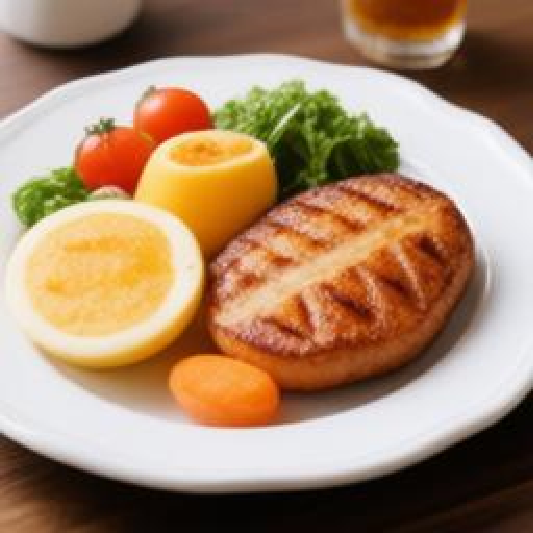
\includegraphics[width=0.24\linewidth]{fig_tab/007749-0112_org_step10_res256.pdf}
        \hfill
        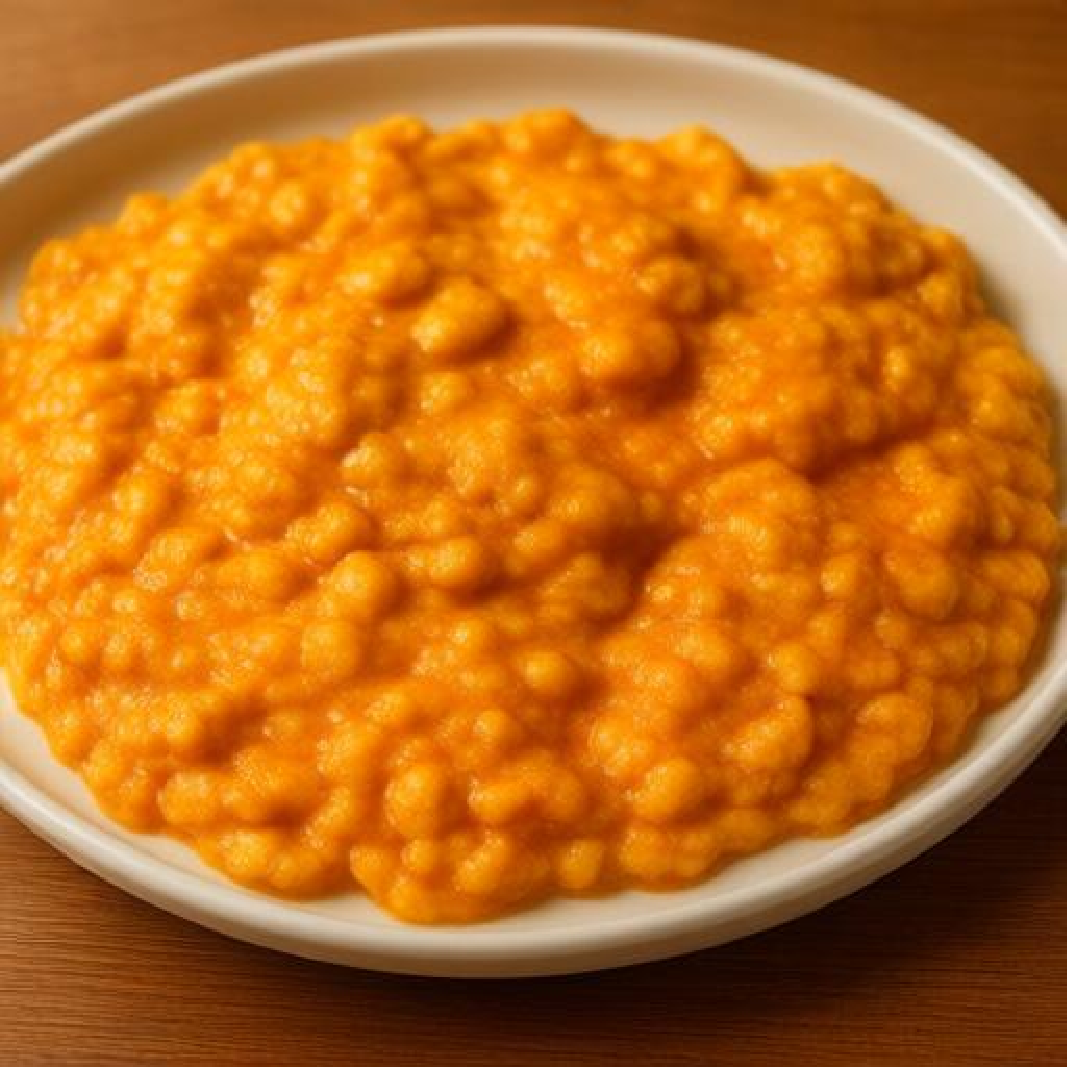
\includegraphics[width=0.24\linewidth]{fig_tab/007749-0112_org_step10_res512.pdf}
        \hfill
        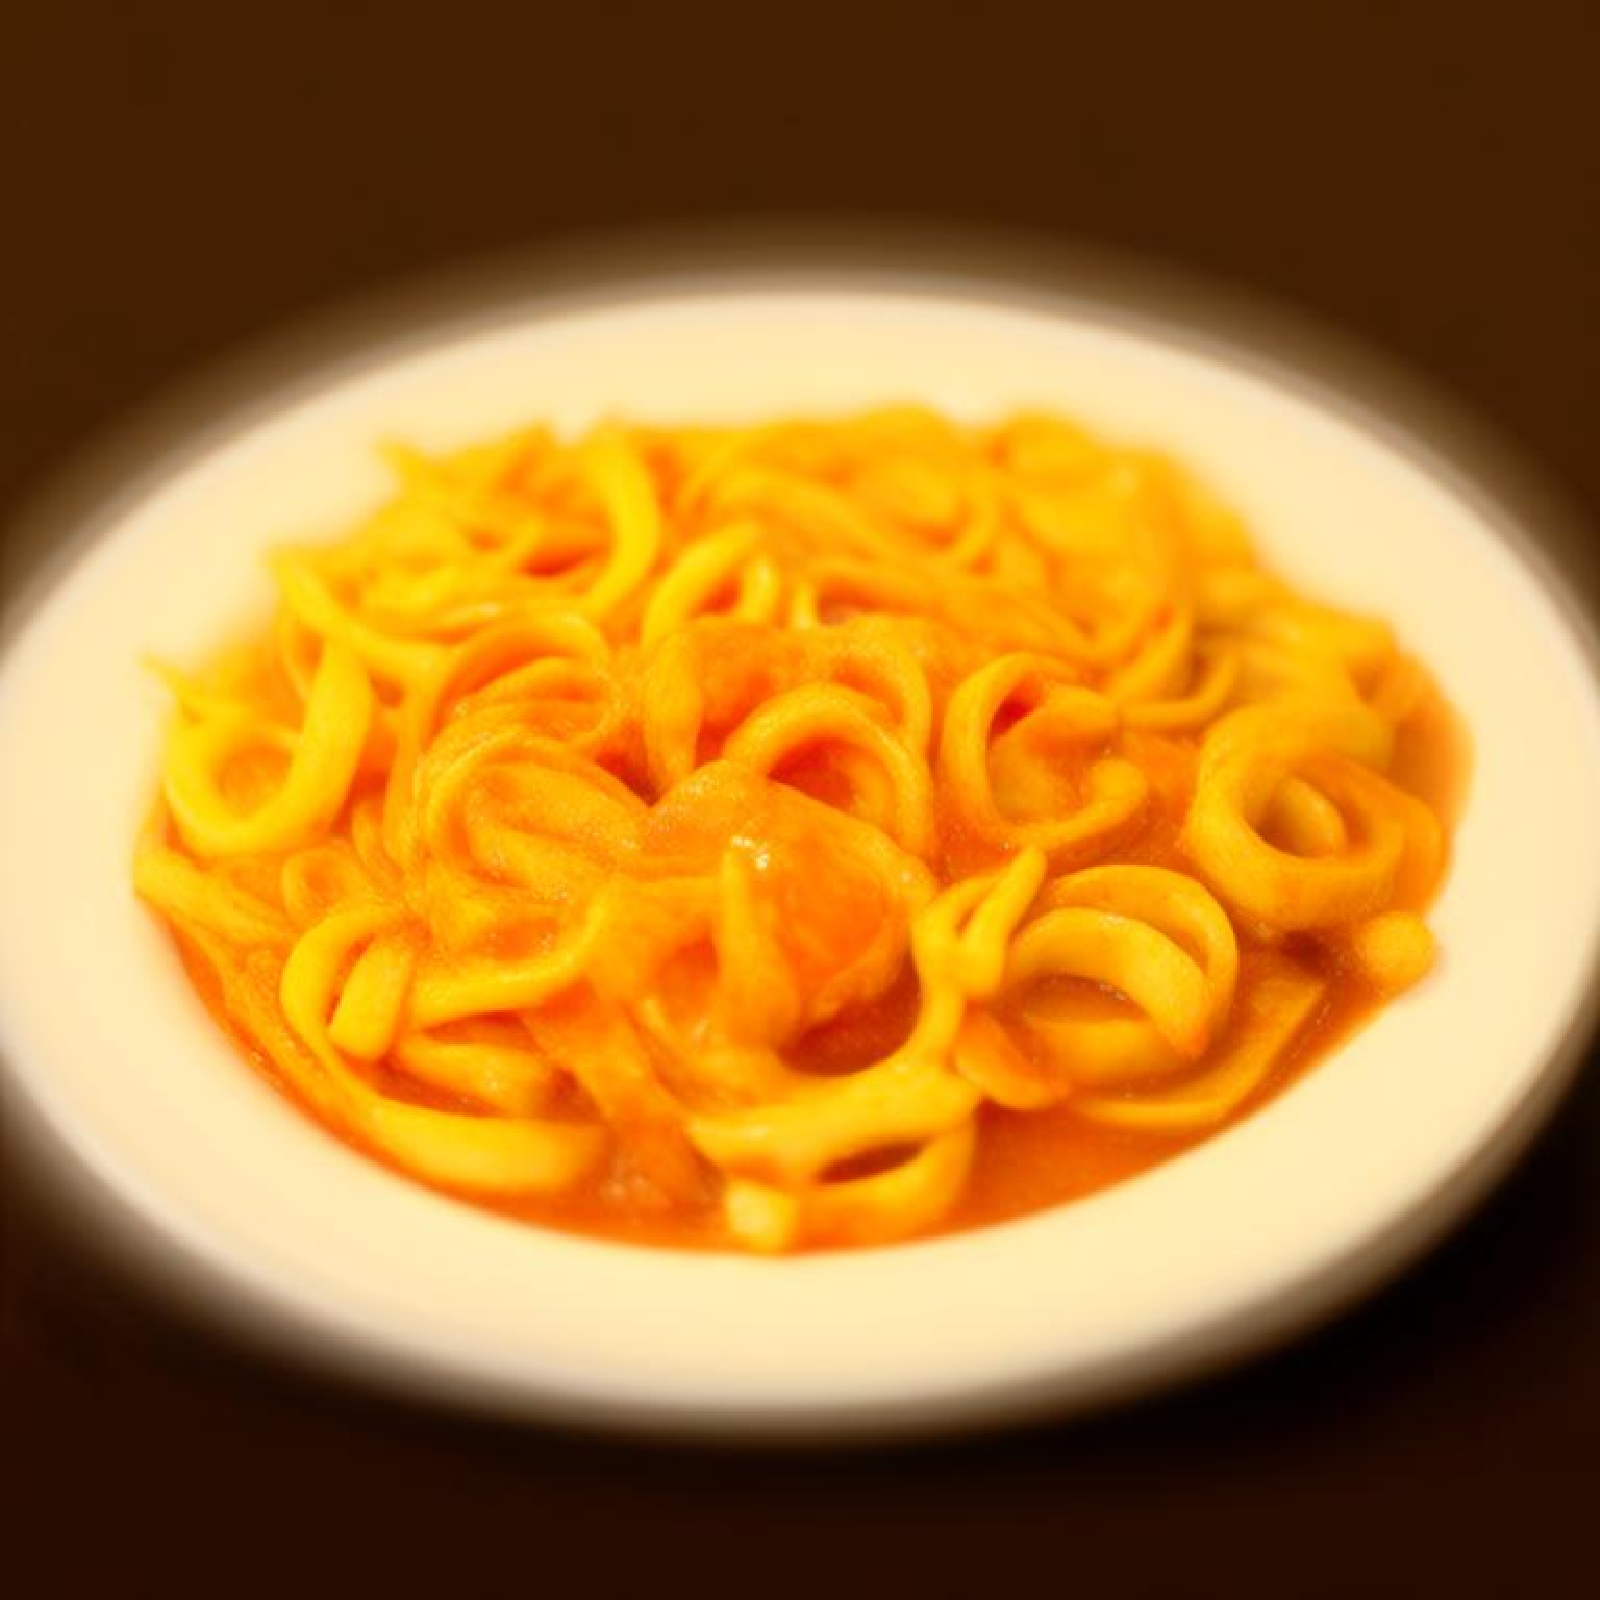
\includegraphics[width=0.24\linewidth]{fig_tab/007749-0112_org_step10_res768.pdf}
        \hfill
        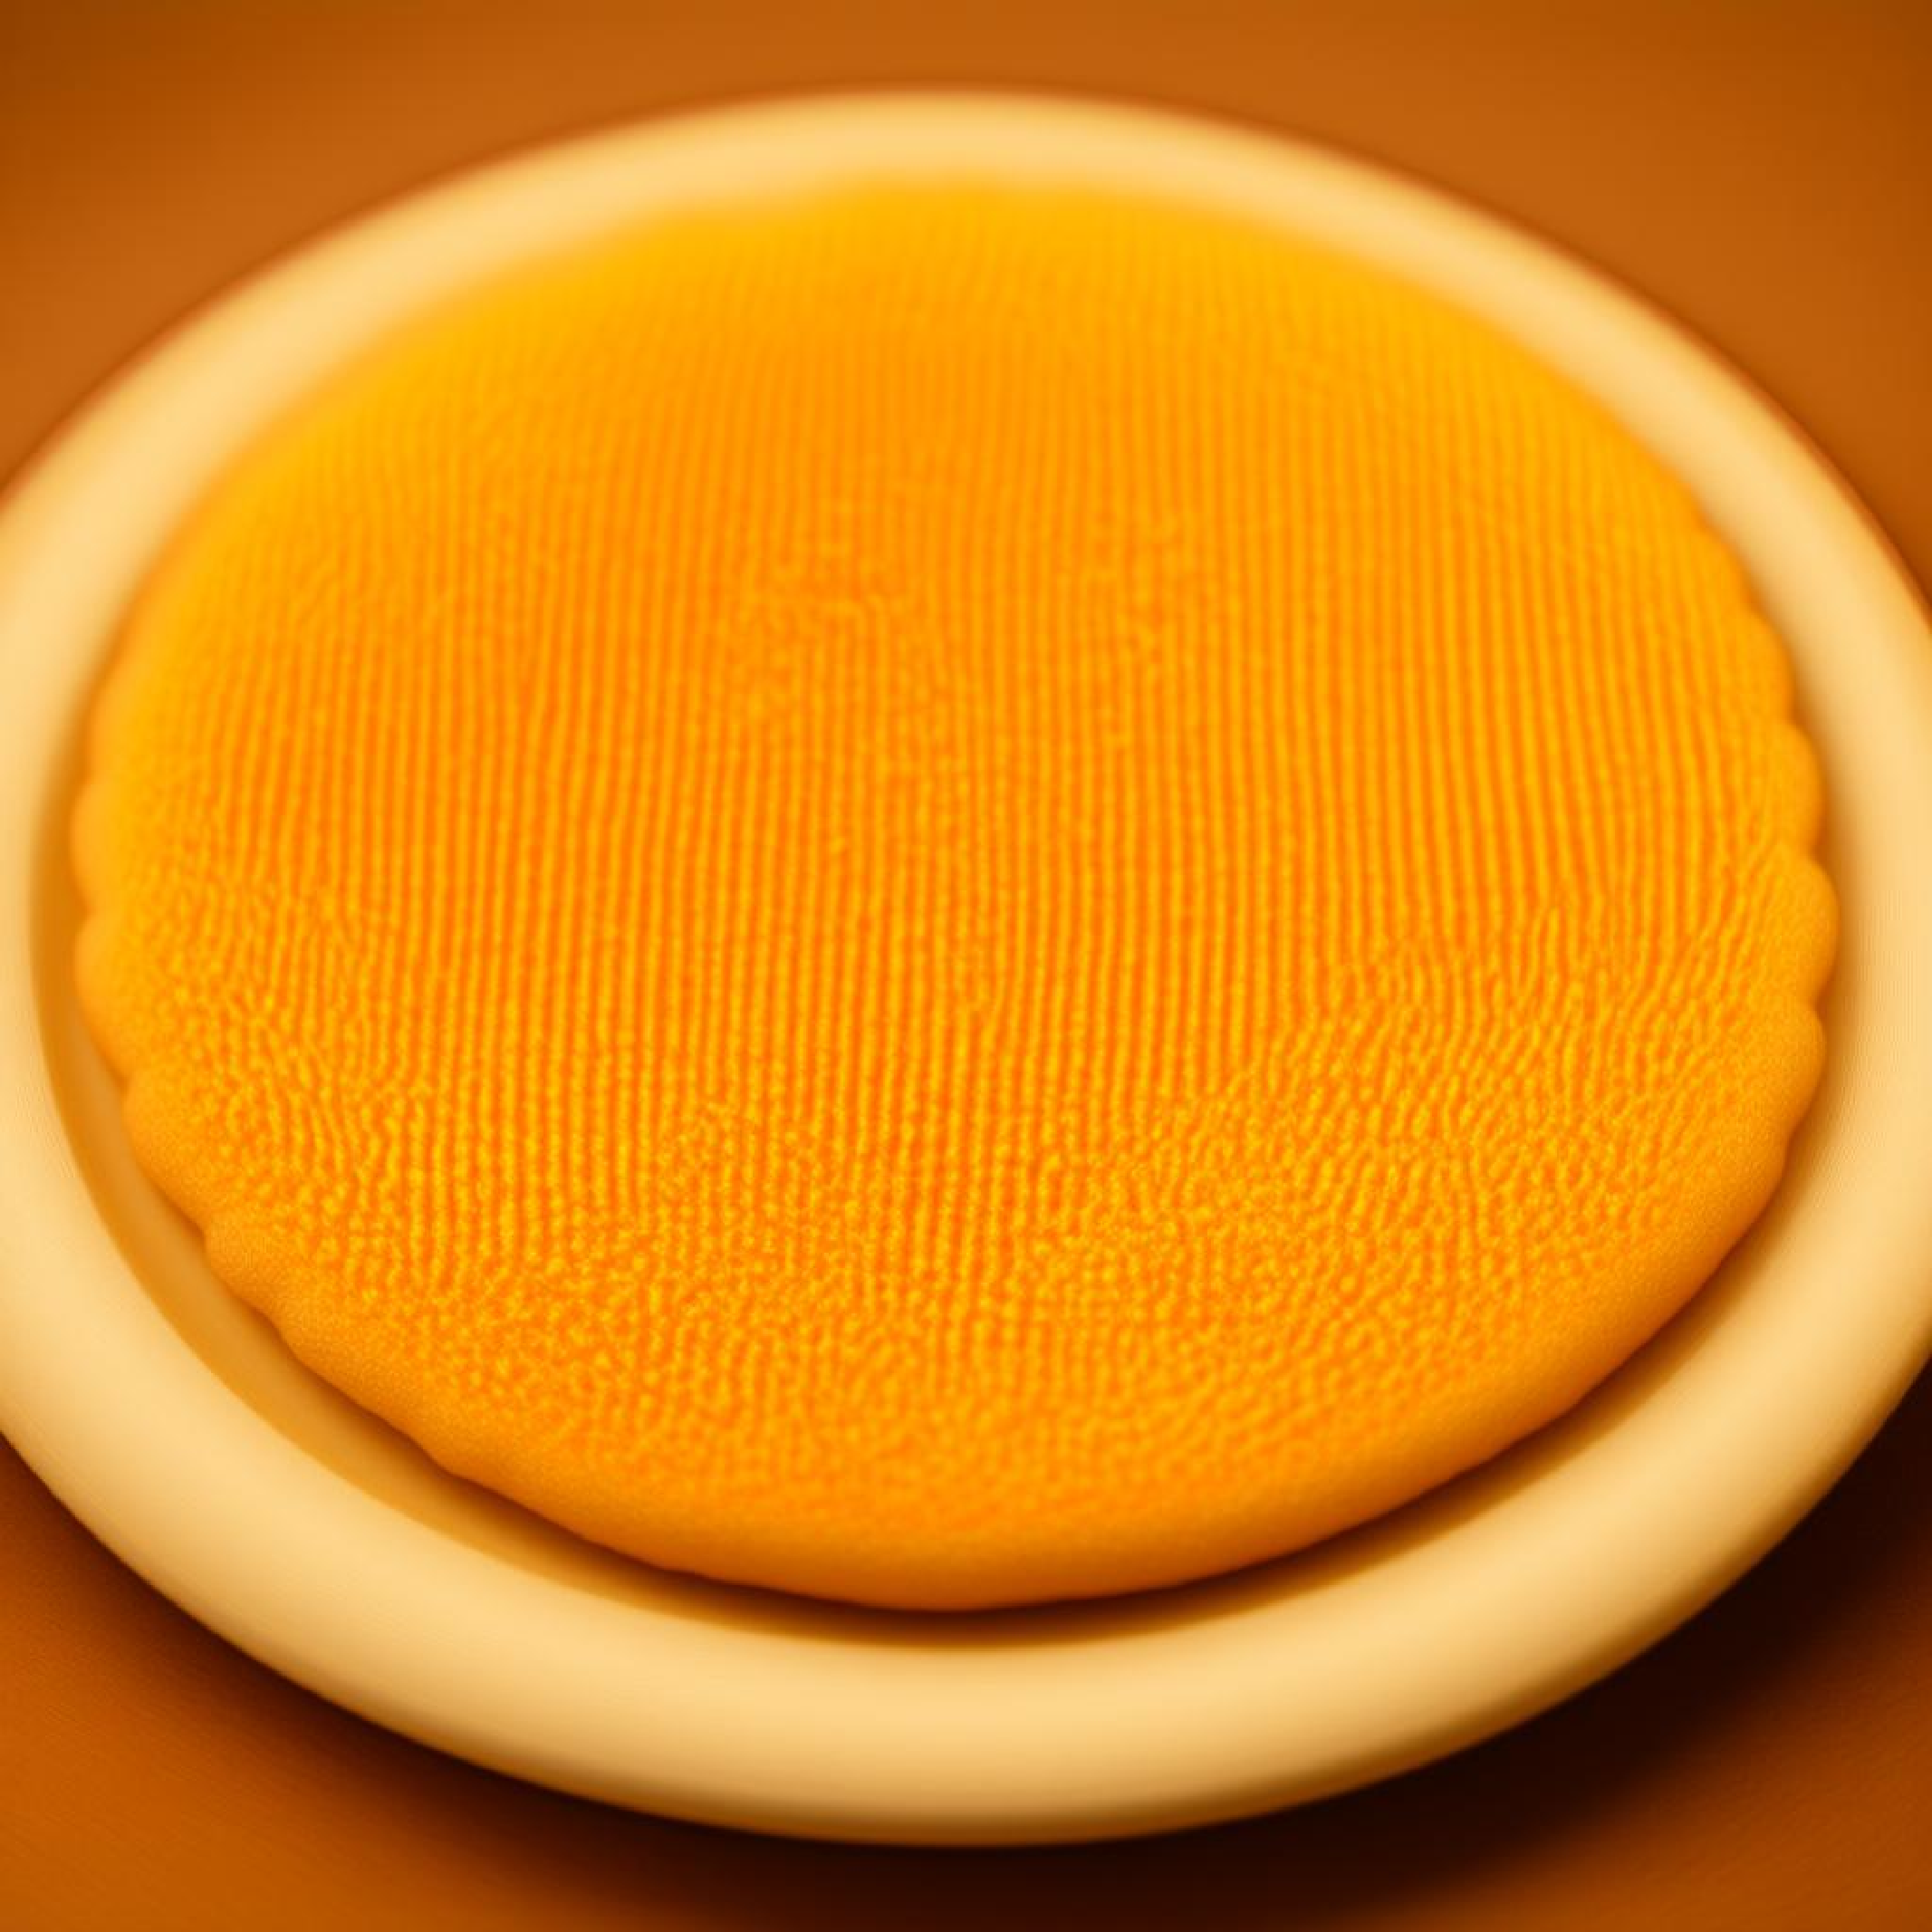
\includegraphics[width=0.24\linewidth]{fig_tab/007749-0112_org_step10_res1024.pdf}
        \caption{Breakfast: Original CFG.}
    \end{subfigure}
    \vspace{2pt}

    % Row 4: Sample 2 (Breakfast) MAMBO-G
    \begin{subfigure}{\linewidth}
        \centering
        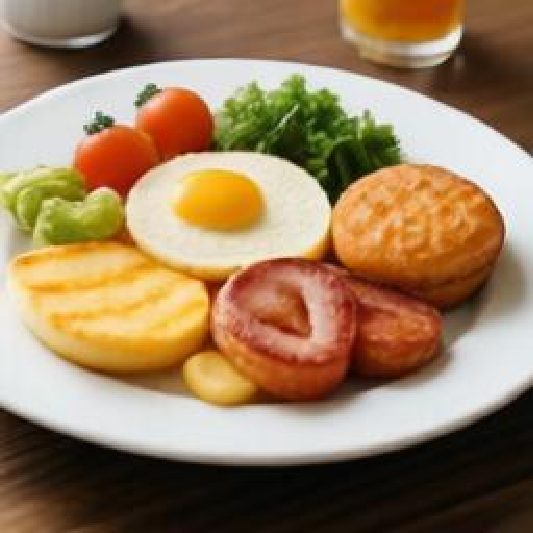
\includegraphics[width=0.24\linewidth]{fig_tab/007749-0112_unify_guidance_step10_res256.pdf}
        \hfill
        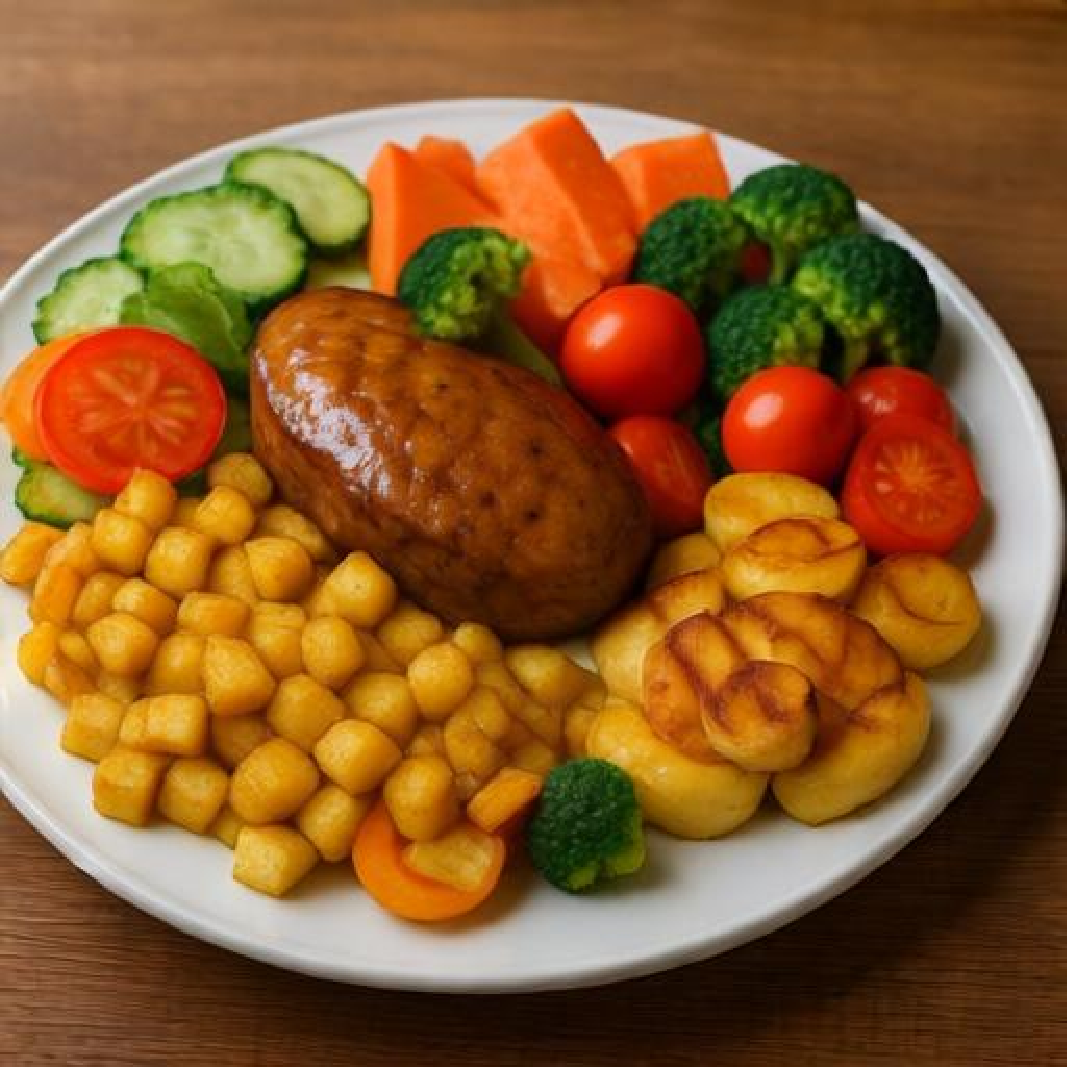
\includegraphics[width=0.24\linewidth]{fig_tab/007749-0112_unify_guidance_step10_res512.pdf}
        \hfill
        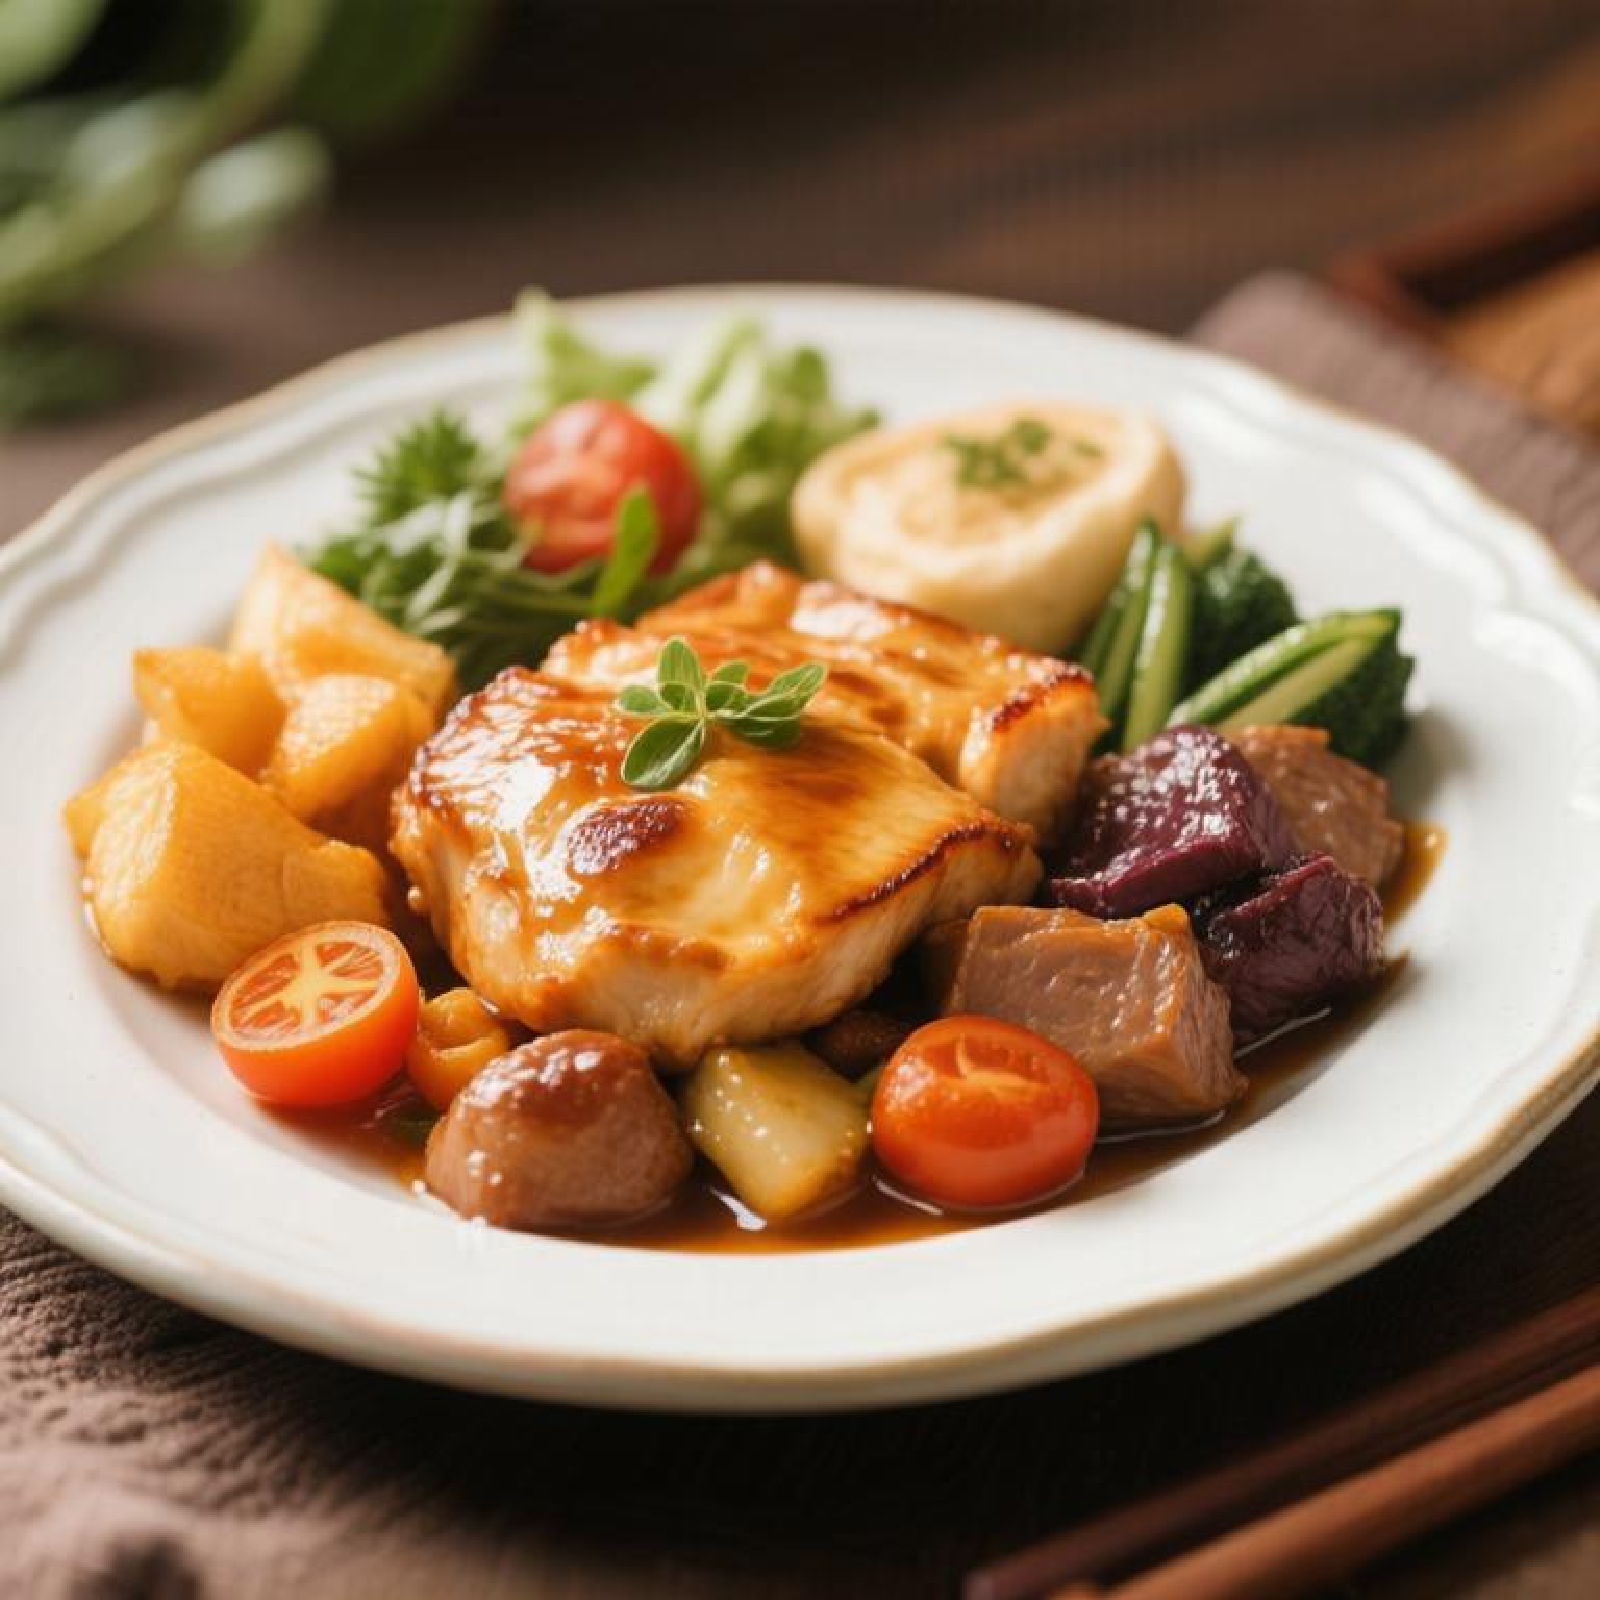
\includegraphics[width=0.24\linewidth]{fig_tab/007749-0112_unify_guidance_step10_res768.pdf}
        \hfill
        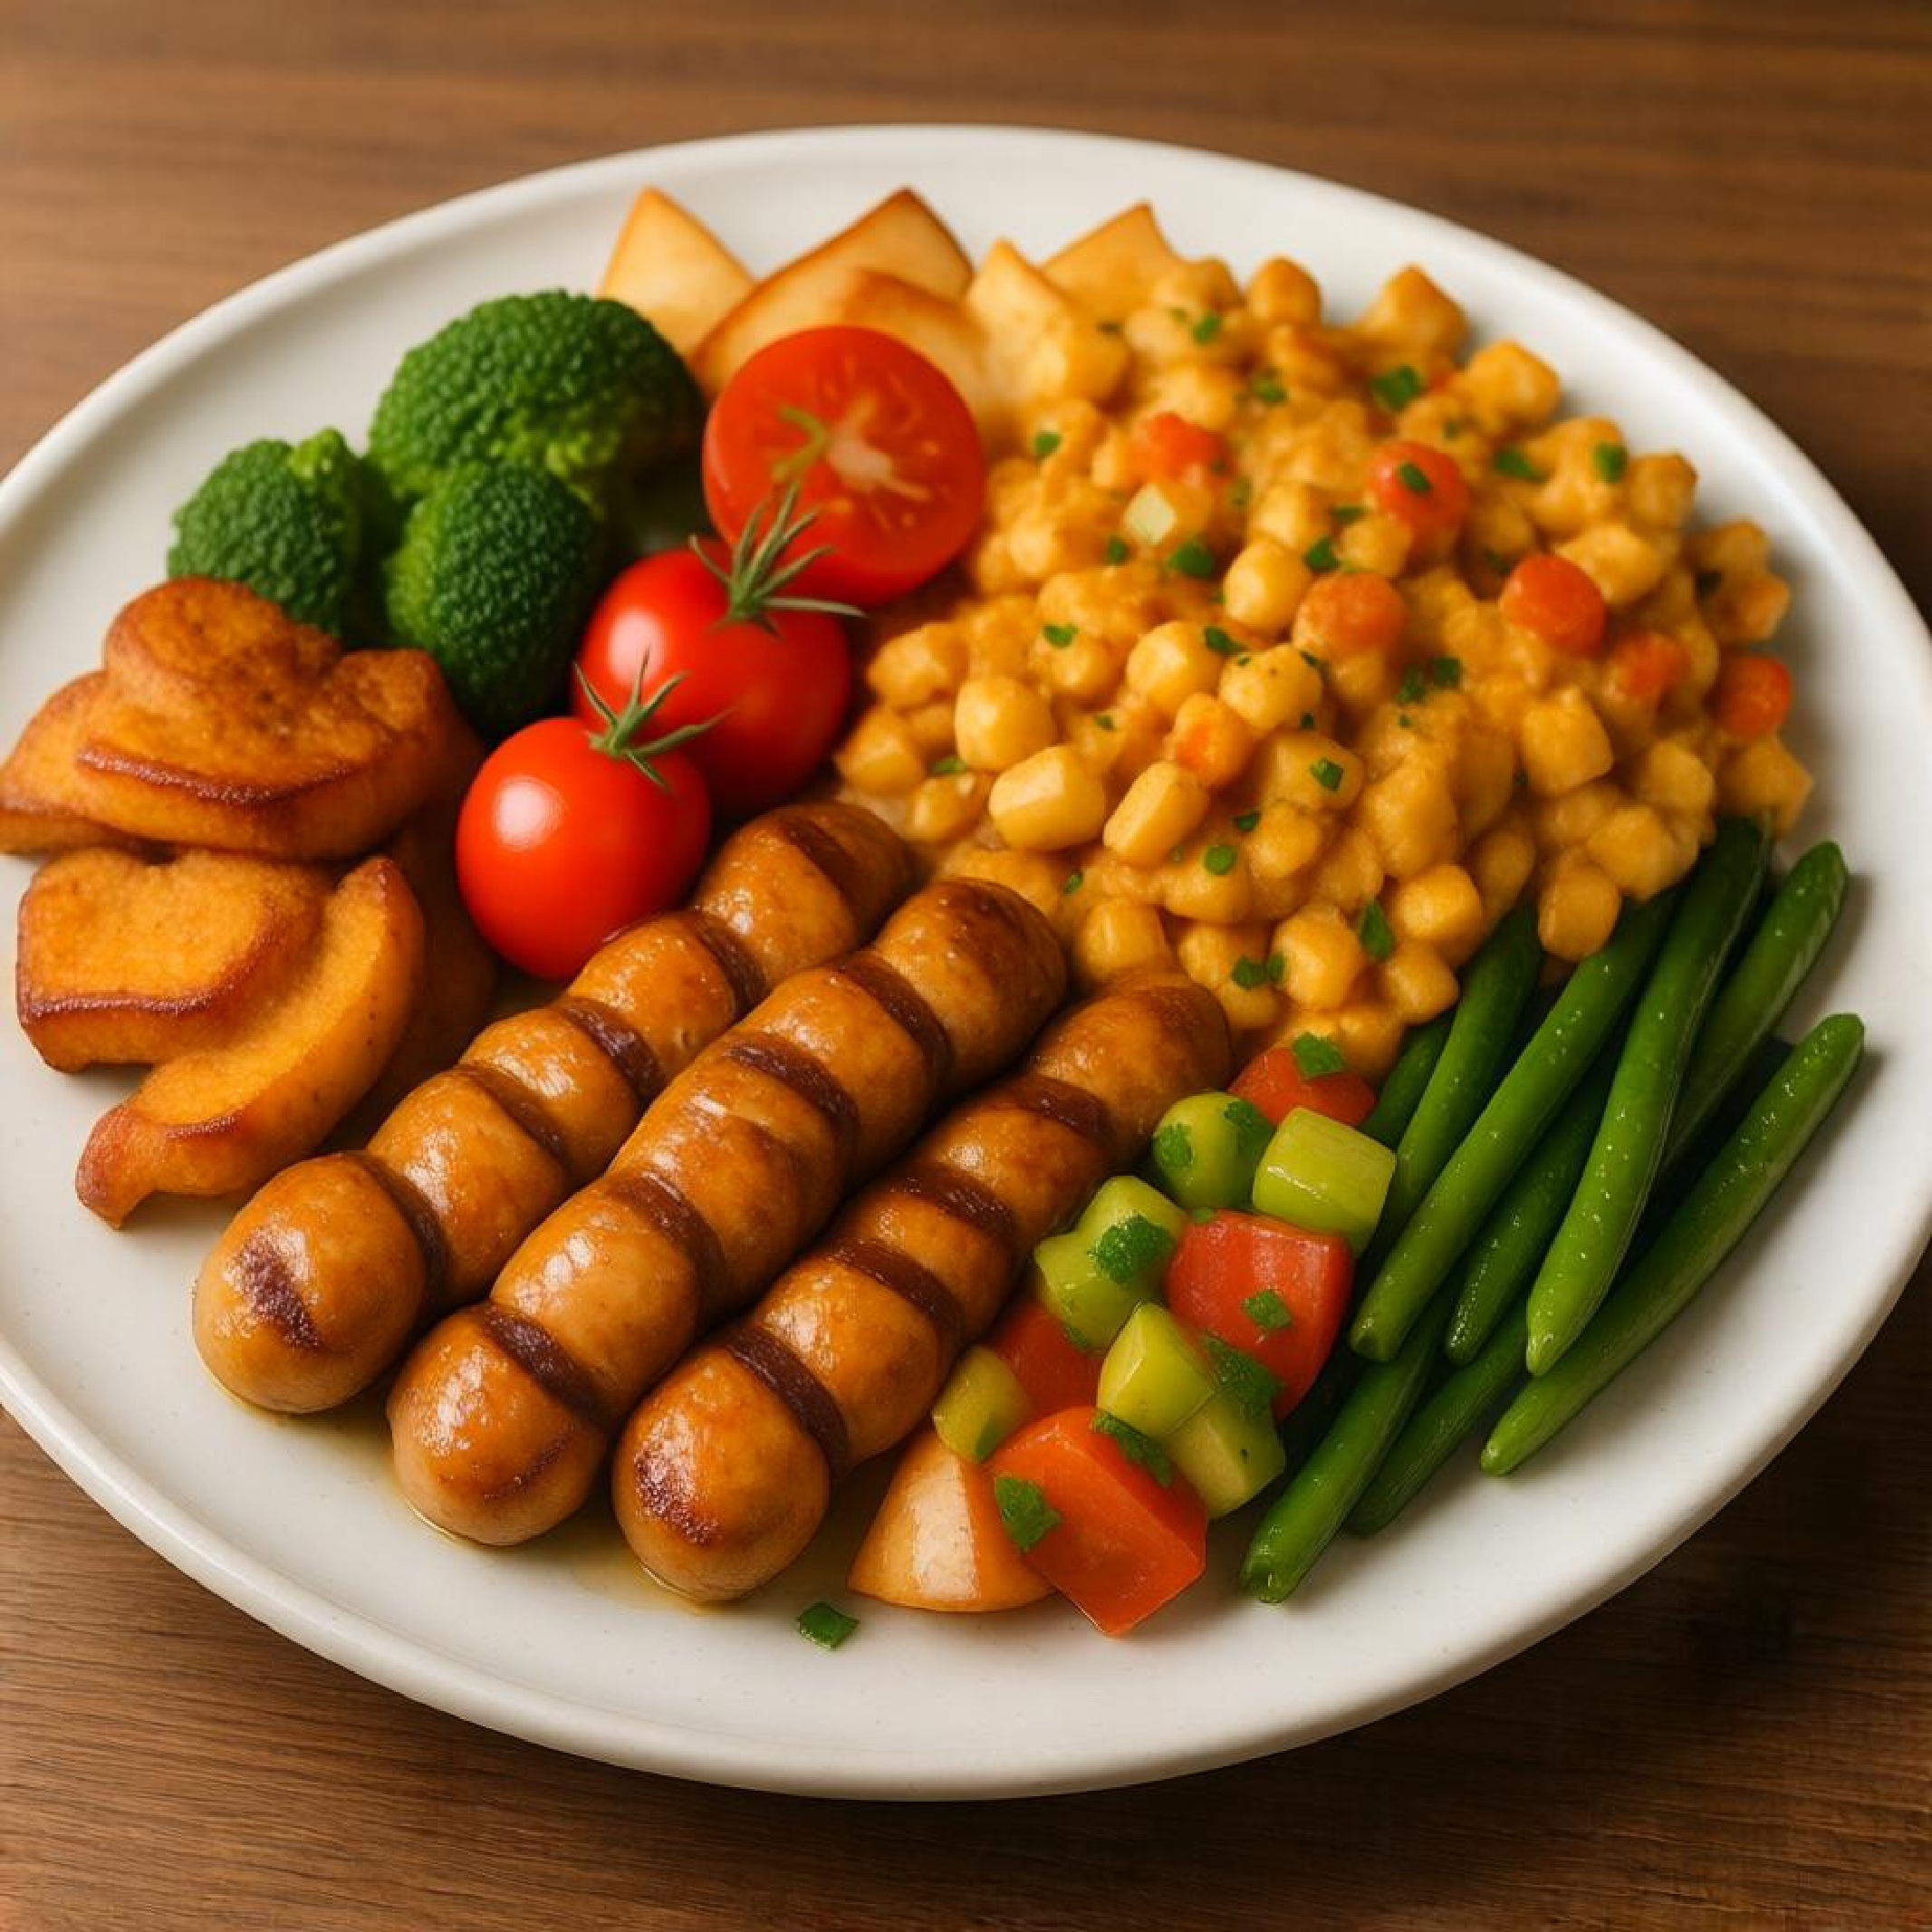
\includegraphics[width=0.24\linewidth]{fig_tab/007749-0112_unify_guidance_step10_res1024.pdf}
        \caption{Breakfast: \mtdbk.}
    \end{subfigure}
    
    \caption{\textbf{Visual comparison across resolutions}: These are Qwen-Image~\citep{wu2025qwen} 10-step samples. From the results, it can be seen that with the original CFG, the higher the resolution, the more unstable the model's sampling results are. With \mtdbk, our method stabilizes the sampling process by adjusting the guidance scale at the instance-level, showing significant improvements.}
    \label{fig:resolution_comparison_4rows}
\end{figure*}